% ~~~~~~~~~~~~~~~~~~~~~~~~~~~~~~~~~~~~~~~~~~~~~~~~~~~~~~~~~~~~~~~~~ %
\newif	\ifexternalize					%\externalizetrue			%
\newif	\ifshowonlynotes				%\showonlynotestrue			%
\newif	\ifhandout						%\handouttrue				%
\newif	\ifshowsolutions				%\showsolutionstrue			%
\newif	\ifshownotes					%\shownotestrue				%
%																	%
% enablers for conditional compiling through bash scripting			%
\ifdefined\EXTERNALIZE	\externalizetrue	\fi						%
\ifdefined\ONLYNOTES	\showonlynotestrue	\fi						%
\ifdefined\HANDOUT		\handouttrue		\fi						%
\ifdefined\SOLUTIONS	\showsolutionstrue	\fi						%
\ifdefined\NOTES		\shownotestrue		\fi						%
%																	%
% ~~~~~~~~~~~~ %
% tab size = 4 %
% ~~~~~~~~~~~~ %

% WARNING: if the compiler returns the error ``incompatible list can't be unboxed''
% try to decomment the following \RequirePackage command:
%\RequirePackage{atbegshi} 

\ifhandout
	\documentclass % ~~~~~~~~~~~~~~~~~~~~~~~~~~~~~~~~~~~~~~~~~~~~~~ %
	[																%
		11pt,														%
		professionalfont,											%
		hyperref={pdfpagelabels=false},								%
		xcolor	={dvipsnames, table},								%
		aspectratio	= 169,											%
		notheorems,													%
		handout,													%
	]																%
	{beamer}														%
	\usepackage{pgfpages}											%
	\ifshownotes													%
		\setbeameroption{show notes}								%
	\fi																%
	\ifshowonlynotes												%
		\setbeameroption{show only notes}							%
	\fi																%
	\pgfpagesuselayout{4 on 1}[a4paper,border shrink=5mm,landscape]	%
\else																%
	\documentclass % ~~~~~~~~~~~~~~~~~~~~~~~~~~~~~~~~~~~~~~~~~~~~~~ %
	[																%
		11pt,														%
		professionalfont,											%
		hyperref={pdfpagelabels=false},								%
		xcolor	={dvipsnames, table},								%
		aspectratio	= 169,											%
		notheorems,													%
	]																%
	{beamer}														%
	\usepackage{pgfpages}											%
	\ifshownotes													%
		\setbeameroption{show notes on second screen=left}			%
	\fi																%
	\ifshowonlynotes												%
		\setbeameroption{show only notes}							%
	\fi																%
\fi																	%
%																	%
% ~~~~~~~~~~~~~~~~~~~~~~~~~~~~~~~~~~~~~~~~~~~~~~~~~~~~~~~~~~~~~~~~~ %
%																	%
\usepackage{etex}													%
\usepackage[english]{babel}											%
\usepackage{type1cm}												%
\usepackage{type1ec}												%
\usepackage[T1]{fontenc}											%
\usepackage{lmodern}												%
\usepackage{amsmath,amssymb,amsfonts,amsthm}						%
\usepackage{graphicx}												%
\usepackage{hyperref}												%
\usepackage{booktabs}												%
\usepackage{bm}														%
\usepackage{dsfont}													%
\usepackage{array}													%
\usepackage{upquote}												%
\usepackage{acronym}												%
\usepackage{MnSymbol}												%
\usepackage[official]{eurosym}										%
\usepackage{xr}														%
\usepackage{varwidth}												%
\usepackage{tikz}													%
\usepackage[european]{circuitikz}									%
\usepackage{enumerate}												%
% \usepackage{enumitem}												%
\usetikzlibrary{shapes.geometric}									%
\usetikzlibrary{positioning}										%
\usetikzlibrary{calc}												%
\usetikzlibrary{matrix}												%
\usetikzlibrary{fit}												%
\usetikzlibrary{arrows.meta}										%
\usetikzlibrary{decorations.text}									%
\newcommand{\figurefilename}[1]{\ifexternalize \tikzsetnextfilename{#1} \fi}
\ifexternalize														%
	\usetikzlibrary{external}										%
	\tikzexternalize[shell escape=-enable-write18]					%
	\tikzset{external/force remake} 								%
\fi																	%
\usepackage{pgfplots}												%
\pgfplotsset{compat=1.14}											%
%																	%
% ~~~~~~~~~~~~~~~~~~~~~~~~~~~~~~~~~~~~~~~~~~~~~~~~~~~~~~~~~~~~~~~~~ %
%																	%
\def\DarkBlue		{black!40!blue}									%
\def\DarkGray		{black!70!white}								%
\def\DarkGreen		{black!40!green}								%
\def\DarkRed		{black!40!red}									%
\def\DarkYellow		{black!40!yellow}								%
\def\DarkOrange		{black!40!orange}								%
%																	%
\def\Blue			{black!10!blue}									%
\def\Gray			{black!50!white}								%
\def\Green			{black!10!green}								%
\def\Red			{black!10!red}									%
\def\Yellow			{black!10!yellow}								%
\def\Orange			{black!10!orange}								%
%																	%
\def\LightBlue		{white!40!blue}									%
\def\LightGray		{white!70!white}								%
\def\LightGreen		{white!40!green}								%
\def\LightRed		{white!40!red}									%
\def\LightYellow	{white!40!yellow}								%
\def\LightOrange	{white!40!orange}								%
%																	%
% ~~~~~~~~~~~~~~~~~~~~~~~~~~~~~~~~~~~~~~~~~~~~~~~~~~~~~~~~~~~~~~~~~ %
%																	%
\def\Background		{white}											%
\def\Foreground		{black}											%
\def\Primary		{Bittersweet!30!red}							%
\def\Secondary		{\Gray}											%
%																	%
\def\StrongPrimary	{\Primary!80!black}								%
\def\SoftPrimary	{\Primary!20!white}								%
\def\StrongSecondary{\Secondary!80!black}							%
\def\SoftSecondary	{\Secondary!20!white}							%
%																	%
% ~~~~~~~~~~~~~~~~~~~~~~~~~~~~~~~~~~~~~~~~~~~~~~~~~~~~~~~~~~~~~~~~~ %
%																	%
\graphicspath{{./Images/}}											%
\everymath{\displaystyle}											%
%																	%

\newcommand{\DefinedAs}			[0]	{\mathrel{\mathop:}=}
\newcommand{\IDefinedAs}		[0]	{=\mathrel{\mathop:}}


\newcommand{\ExponentialOf}		[1]	{\mathrm{exp} \left( #1 \right)}
\newcommand{\LogarithmOf}		[1]	{\mathrm{log} \left( #1 \right)}
\newcommand{\ConvexHullOf}		[1]	{\mathrm{c.h.} \left( #1 \right)}


\newcommand{\MaximumOfOne}		[1]	{\mathrm{max} \left\lbrace #1 \right\rbrace}
\newcommand{\MaximumOfTwo}		[2]	{\mathrm{max} \left\lbrace #1, #2 \right\rbrace)}
\newcommand{\MaximumOfThree}	[3]	{\mathrm{max} \left\lbrace #1, #2, #3 \right\rbrace)}
\newcommand{\MinimumOfOne}		[1]	{\mathrm{min} \left\lbrace #1 \right\rbrace}
\newcommand{\MinimumOfTwo}		[2]	{\mathrm{min} \left\lbrace #1, #2 \right\rbrace)}
\newcommand{\MinimumOfThree}	[3]	{\mathrm{min} \left\lbrace #1, #2, #3 \right\rbrace)}


\newcommand{\CostFunction}				[0]	{Q}
\newcommand{\CostFunctionOf}			[1]	{\CostFunction \left( #1 \right)}
\newcommand{\CostFunctionOfSensor}		[1]	{\CostFunction_{#1}}
\newcommand{\CostFunctionOfSensorOf}	[2]	{\CostFunctionOfSensor{#1} \left( #2 \right)}


\newcommand{\KroneckerDeltaOf}			[2]	{\delta_{#1 #2}}


\newcommand{\FloorOf}			[1]	{\lfloor #1 \rfloor}
\newcommand{\CeilOf}			[1]	{\lceil #1 \rceil}


\newcommand{\GammaFunctionOf}	[1]	{\Gamma \left( #1 \right)}

\newcommand{\IdentityMatrix}		[1]	{I_{#1}}
\newcommand{\OnesVector}			[1]	{\mathds{1}_{#1}}

\newcommand{\TraceOf}				[1]	{\text{tr} \left( #1 \right)}
\newcommand{\DeterminantOf}			[1]	{\text{det} \left( #1 \right)}
\newcommand{\SetOfEigenvaluesOf}	[1]	{\text{eig} \left( #1 \right)}

\newcommand{\Eigenvalue}			[1]	{\lambda_{#1}}
\newcommand{\Eigenvector}			[1]	{v_{#1}}
\newcommand{\MaximalEigenvalue}		[0]	{\lambda_{\text{max}}}
\newcommand{\MinimalEigenvalue}		[0]	{\lambda_{\text{min}}}

\newcommand{\SpectralRadius}		[0]	{\mu}
\newcommand{\SpectralRadiusOf}		[1]	{\SpectralRadius \left( #1 \right)}


\newcommand{\GaussianDistribution}					[2]	{\mathcal{N} \left( #1, #2 \right)}
\newcommand{\GammaDistribution}						[2]	{\text{Gamma} \left( #1, #2 \right)}
\newcommand{\ChiSquareDistribution}					[0]	{\chi^{2}}
\newcommand{\ChiSquareDistributionOfIndex}			[1]	{\ChiSquareDistribution \left( #1 \right)}
\newcommand{\InverseChiSquareDistribution}			[0]	{\text{Inv-}\chi^{2}}
\newcommand{\InverseChiSquareDistributionOfIndex}	[1]	{\InverseChiSquareDistribution \left( #1 \right)}
\newcommand{\UniformDistribution}					[2]	{\mathcal{U} \left[ #1, #2 \right]}
\newcommand{\ExponentialDistribution}				[1]	{\text{Exp} \left( #1 \right)}


\newcommand{\Reals}						[0]	{\mathbb{R}}
\newcommand{\PositiveReals}				[0]	{\mathbb{R}_{+}}
\newcommand{\Naturals}					[0]	{\mathbb{N}}
\newcommand{\PositiveNaturals}			[0]	{\mathbb{N}_{+}}

\newcommand{\SetOfSquareSummableInfiniteVectors}			[0]	{\ell}
\newcommand{\SetOfWeightedSquareSummableInfiniteVectors}	[0]	{\textsl{l}_{\RKHS}}
\newcommand{\SetOfSquareIntegrableFunctions}				[0]	{\textsl{L}^{2}}
\newcommand{\SetOfSquareIntegrableFunctionsIn}				[1]	{\textsl{L}^{2} \left( #1 \right)}

\newcommand{\Probability}			[0]	{\mathbb{P}}
\newcommand{\ProbabilityOf}			[1]	{\Probability \left[ #1 \right]}
\newcommand{\ProbabilityOfGiven}	[2]	{\ProbabilityOf{ #1 \; \left| \; #2 \right.}}


\newcommand{\ProbabilityDistribution}		[0]	{P}
\newcommand{\ProbabilityDistributionOf}		[1]	{\ProbabilityDistribution \left( #1 \right)}
\newcommand{\ProbabilityDistributionOfGiven}[2]	{\ProbabilityDistributionOf{ #1 \left| #2 \right. }}
%
\newcommand{\ProbabilityDistributionOfRV}	[1]	{\ProbabilityDistribution_{#1}}
\newcommand{\ProbabilityDistributionOfRVOf}	[2]	{\ProbabilityDistributionOfRV{#1} \left( #2 \right)}
\newcommand{\ProbabilityDistributionOfRVOfGiven}	[3]
		   {\ProbabilityDistributionOfRVOf{#1}{ #2 \left| #3 \right. }}


\newcommand{\ProbabilityDensity}			[0]	{p}
\newcommand{\ProbabilityDensityOf}			[1]	{\ProbabilityDensity \left( #1 \right)}
\newcommand{\ProbabilityDensityOfGiven}		[2]	{\ProbabilityDensityOf{ #1 \left| #2 \right. }}
%
\newcommand{\ProbabilityDensityOfRV}		[1]	{\ProbabilityDensity_{#1}}
\newcommand{\ProbabilityDensityOfRVOf}		[2]	{\ProbabilityDensityOfRV{#1} \left( #2 \right)}
\newcommand{\ProbabilityDensityOfRVOfGiven}	[3] {\ProbabilityDensityOfRVOf{#1}{ #2 \left| #3 \right. }}


\newcommand{\ProbabilityMassFunction}		[0]	{m}
\newcommand{\ProbabilityMassFunctionOf}		[1]	{\ProbabilityMassFunction \left( #1 \right)}
\newcommand{\ProbabilityMassFunctionOfGiven}[2]	{\ProbabilityMassFunctionOf{ #1 \left| #2 \right. }}
%
\newcommand{\ProbabilityMassFunctionOfRV}	[1]	{\ProbabilityMassFunction_{#1}}
\newcommand{\ProbabilityMassFunctionOfRVOf}	[2]	{\ProbabilityMassFunctionOfRV{#1} \left( #2 \right)}
\newcommand{\ProbabilityMassFunctionOfRVOfGiven}		[3]
		   {\ProbabilityMassFunctionOfRVOf{#1}{ #2 \left| #3 \right. }}


\newcommand{\Expectation}					[0]	{\mathbb{E}}
\newcommand{\ExpectationOf}					[1]	{\Expectation \left[ #1 \right]}
\newcommand{\ExpectationOfOnMeasure}		[2]	{\Expectation_{#2} \left[ #1 \right]}
\newcommand{\ExpectationOfGiven}			[2]	{\ExpectationOf{ #1 \; \left| \; #2 \right. }}
\newcommand{\ExpectationOfOnMeasureGiven}	[3]	{\ExpectationOfOnMeasure{#1 \; \left| \; #3 \right.}{#2}}


\newcommand{\Variance}				[0]	{\mathrm{var}}
\newcommand{\VarianceOf}			[1]	{\Variance \left( #1 \right)}
\newcommand{\VarianceOfGiven}		[2]	{\VarianceOf{ #1 \; \left| \; #2 \right. }}


\newcommand{\Covariance}			[0]	{\mathrm{cov}}
\newcommand{\CovarianceOf}			[2]	{\Covariance \left( #1, #2 \right)}
\newcommand{\CovarianceOfGiven}		[3]	{\Covariance \left( #1, #2 \; \left| \; #3 \right. \right)}


\newcommand{\BayesEstimatorOfGiven}	[2]	{\widehat{\Expectation} \left[ #1 \; \left| \; #2 \right. \right] }


\newcommand{\IndicatorFunctionOf}	[1]	{\mathds{1} \left\lbrace #1 \right\rbrace}


\newcommand{\SufficientStatistic}	[0]	{T}
\newcommand{\SufficientStatisticOf}	[1]	{\SufficientStatistic \left( #1 \right)}

\newcommand{\Fingers}
{
	\begin{itemize}
		\item yes \hfill (1 finger)
		\item yes, maybe \hfill (2 fingers)
		\item I don't know \hfill (3 fingers)
		\item no, maybe not \hfill (4 fingers)
		\item no \hfill (5 fingers)
	\end{itemize}
}

\newcommand	{\SuchThat}				{s.t.\ }

\newcommand	{\Section}				[0]	{Sec.}
\newcommand	{\Sections}				[0]	{Secc.}
\newcommand	{\Equation}				[0]	{Equ.}
\newcommand	{\Equations}			[0]	{Equu.}
\newcommand	{\Figure}				[0]	{Fig.}
\newcommand	{\Figures}				[0]	{Figg.}
\newcommand	{\Table}				[0]	{Tab.}
\newcommand	{\Tables}				[0]	{Tabb.}
\newcommand	{\Algorithm}			[0]	{Alg.}
\newcommand	{\Algorithms}			[0]	{Algg.}
\newcommand	{\Proposition}			[0]	{Prop.}
\newcommand	{\Propositions}			[0]	{Propp.}
\newcommand	{\Hypothesis}			[0]	{Hyp.}
\newcommand	{\Hypotheses}			[0]	{Hypp.}

\setbeamertemplate{theorems}[numbered]
\newtheorem{question}{Question}

\newcounter{QuestionsCounter}
\stepcounter{QuestionsCounter}

\newcommand	{\QuestionID}		[1]	{\JustSecondary{(ID: #1)} \label{question:#1} \stepcounter{QuestionsCounter}}
\newcommand	{\QuestionKCs}		[1] {}
\newcommand	{\QuestionKCsTaxonomies}	[1] {}
\newcommand	{\QuestionNotes}	[1] {}
\newcommand	{\QuestionBody}		[1] {#1}
\newcommand	{\QuestionImage}	[2] {\begin{center} \includegraphics[#1]{#2} \end{center}}
\newcommand	{\QuestionAnswers}	[1] {\begin{enumerate} #1 \end{enumerate}}
\newcommand	{\QuestionSolution}	[1] {\ifshowsolutions \note<1->{#1} \fi}
\newcommand	{\QuestionAuthor}	[1] {}
\newcommand	{\QuestionVersion}	[1] {}







\newcommand{\answer}		[0]
{
	\item[\addtocounter{enumi}{1} \tikz{ \node [anchor = base, baseline, minimum width = 0.6cm, minimum height = 0.6cm, draw] {\arabic{enumi}};}]
}

\newcommand{\correctanswer}	[0]
{
	\ifshowsolutions
		\item[\addtocounter{enumi}{1} \tikz{ \node [anchor = base, baseline, minimum width = 0.6cm, minimum height = 0.6cm, draw, fill = red!30!white] {\arabic{enumi}};}]
	\else
		\answer
	\fi
}

% \newcommand{\hideableanswer}[1]{\item \ifshowsolutions #1 \fi}





\pgfdeclarelayer{ultrabackground}
\pgfdeclarelayer{background}
\pgfdeclarelayer{foreground}
\pgfsetlayers{ultrabackground,background,main,foreground}
% \begin{pgfonlayer}{background} 
% \end{pgfonlayer}


\newcommand{\JustPrimary}		[1]{\textcolor{\StrongPrimary}{#1}}
\newcommand{\ItPrimary}			[1]{\textcolor{\StrongPrimary}{\textit{#1}}}
\newcommand{\BoldPrimary}		[1]{\textcolor{\StrongPrimary}{\textbf{#1}}}
\newcommand{\BoldItPrimary}		[1]{\textcolor{\StrongPrimary}{\textit{ \textbf{#1} }}}
\newcommand{\ItBoldPrimary}		[1]{\BoldItPrimary{#1}}
\newcommand{\MathBoxPrimary}	[1]{\colorbox{\SoftPrimary}{#1}}
%
\newcommand{\JustSecondary}		[1]{\textcolor{\StrongSecondary}{#1}}
\newcommand{\ItSecondary}		[1]{\textcolor{\StrongSecondary}{\textit{#1}}}
\newcommand{\BoldSecondary}		[1]{\textcolor{\StrongSecondary}{\textbf{#1}}}
\newcommand{\BoldItSecondary}	[1]{\textcolor{\StrongSecondary}{\textit{ \textbf{#1} }}}
\newcommand{\ItBoldSecondary}	[1]{\BoldItSecondary{#1}}
\newcommand{\MathBoxSecondary}	[1]{\colorbox{\SoftSecondary}{#1}}
%
\newcommand{\Code}				[1]{\texttt{\textcolor{\StrongSecondary}{#1}}}


\newcommand{\NewSection}		[1]
{
	\subsection{#1}
	\label{sec: #1}
	\setbeamercolor{background canvas}{bg=\SoftPrimary}
	\begin{frame}
		\begin{center}
			\Large #1
		\end{center}
		\note<1-1>{\begin{itemize}
			\item 
		\end{itemize}}
	\end{frame}
	\setbeamercolor{background canvas}{bg=white}
}

\newcommand{\QuestionMark}		[0]
{
	\setbeamercolor{background canvas}{bg=\SoftSecondary}
	\begin{frame}
		\begin{center}
			\Large ?
		\end{center}
		\note<1-1>{\begin{itemize}
			\item 
		\end{itemize}}
	\end{frame}
	\setbeamercolor{background canvas}{bg=white}
}

\newcommand {\PrimaryRectangle} [1]
{
	\begin{center}
	\begin{tikzpicture}
		%
		\node
		[
			shape			= rectangle,		% shape
			rounded corners	= 0.2cm,			% shape
			minimum width	= 0.7cm,			%
			minimum height	= 0.7cm,			%
			line width		= 0cm,				% thickness of the border
			fill			= \SoftPrimary,		%
			draw			= \StrongPrimary,	% draw the border with this color
			line width		= 0.1cm,			% thickness
			text width		= 0.8\textwidth,	% max. width of the text
			align			= center,			% text alignment
			inner xsep		= 0.2cm,			%
			inner ysep		= 0.2cm,			%
		]
		{#1};
		%
	\end{tikzpicture}
	\end{center}
}

\newcommand {\SecondaryRectangle} [1]
{
	\begin{center}
	\begin{tikzpicture}
		%
		\node
		[
			shape			= rectangle,		% shape
			rounded corners	= 0.2cm,			% shape
			minimum width	= 0.7cm,			%
			minimum height	= 0.7cm,			%
			line width		= 0cm,				% thickness of the border
			fill			= \SoftSecondary,	%
			draw			= \StrongSecondary,	% draw the border with this color
			line width		= 0.1cm,			% thickness
			text width		= 0.9\textwidth,	% max. width of the text
			align			= center,			% text alignment
			inner xsep		= 0.2cm,			%
			inner ysep		= 0.2cm,			%
		]
		{#1};
		%
	\end{tikzpicture}
	\end{center}
}

\newcommand {\PrimaryRectangleWithCaption} [3]
{
	\begin{center}
	\begin{tikzpicture}
		%
		\node (a)
		[
			shape			= rectangle,		% shape
			rounded corners	= 0.2cm,			% shape
			minimum width	= 0.7cm,			%
			minimum height	= 0.7cm,			%
			fill			= \SoftPrimary,		%
			draw			= \StrongPrimary,	% draw the border with this color
			line width		= 0.1cm,			% thickness
			text width		= 0.8\textwidth,	% max. width of the text
			align			= center,			% text alignment
			inner xsep		= 0.3cm,			%
			inner ysep		= 0.3cm,			%
		]
		{#2};
		%
		\node
		[
			shape			= rectangle,		% shape
			rounded corners	= 0.2cm,			% shape
			anchor			= mid,
			fill			= \SoftPrimary,		%
			draw			= \StrongPrimary,	% draw the border with this color
			text			= \StrongPrimary,	%
			align			= center,			% text alignment
			line width		= 0.1cm,			% thickness
			inner xsep		= 0.2cm,			%
			inner ysep		= 0.2cm,			%
		]
		at (a.#3)
		{#1};
		%
	\end{tikzpicture}
	\end{center}
}

\newcommand {\SecondaryRectangleWithCaption} [3]
{
	\begin{center}
	\begin{tikzpicture}
		%
		\node (a)
		[
			shape			= rectangle,		% shape
			rounded corners	= 0.2cm,			% shape
			minimum width	= 0.7cm,			%
			minimum height	= 0.7cm,			%
			fill			= \SoftSecondary,	%
			draw			= \StrongSecondary,	% draw the border with this color
			line width		= 0.1cm,			% thickness
			text width		= 0.8\textwidth,	% max. width of the text
			align			= center,			% text alignment
			inner xsep		= 0.3cm,			%
			inner ysep		= 0.3cm,			%
		]
		{#2};
		%
		\node
		[
			shape			= rectangle,		% shape
			rounded corners	= 0.2cm,			% shape
			anchor			= mid,
			fill			= \SoftSecondary,	%
			draw			= \StrongSecondary,	% draw the border with this color
			text			= \StrongSecondary,	%
			align			= center,			% text alignment
			line width		= 0.1cm,			% thickness
			inner xsep		= 0.2cm,			%
			inner ysep		= 0.2cm,			%
		]
		at (a.#3)
		{#1};
		%
	\end{tikzpicture}
	\end{center}
}

\newcommand{\InsertImage}[3] % path / height / width
{
	\begin{tikzpicture}[remember picture, overlay]
	\node
	[
		shape			= rectangle,		% shape
		minimum height	= #2cm,				% | minimum size of the node
		minimum width	= #3cm,				% |
 		path picture	=
		{\node at (path picture bounding box.center)
		{\includegraphics[height = #2cm, width = #3cm]
		{#1}};}
	]{};
	\end{tikzpicture}
}

\newcommand{\InsertImageAt}[5] % path / height / width / xshift / yshift
{
	\begin{tikzpicture}[remember picture, overlay]
	\node
	[
		shape			= rectangle,		% shape
		minimum height	= #2cm,				% | minimum size of the node
		minimum width	= #3cm,				% |
		xshift 			= #4cm,
		yshift			= #5cm,
 		path picture	=
		{\node at (path picture bounding box.center)
		{\includegraphics[height = #2cm, width = #3cm]
		{#1}};}
	]
	at (current page.center)
	{};
	\end{tikzpicture}
}

\newcommand{\InsertTextAt}[3] % text / xshift / yshift
{
	\begin{tikzpicture}[remember picture, overlay]
	\node
	[
		shape			= rectangle,		% shape
		xshift 			= #2cm,
		yshift			= #3cm,
	]
	at (current page.center)
	{#1};
	\end{tikzpicture}
}

\newcommand{\Formula}[2]
{
	\begin{frame}[t]
	\ifexternalize
		\tikzsetnextfilename{formula-#1}
	\fi
	\begin{tikzpicture}
		\node
		{$
			#2
		$};
	\end{tikzpicture}
	\end{frame}
}

										%
\pgfdeclarelayer{ultrabackground}
\pgfdeclarelayer{background}
\pgfdeclarelayer{foreground}
\pgfsetlayers{ultrabackground,background,main,foreground}

\tikzset
{
	FancyCircle/.style =
	{
		shape					= circle,
		line width				= 0.1cm,
		align					= center,
		inner xsep				= 0.1cm,
		inner ysep				= 0.1cm,
		text width				= 2.4cm,
%		circular drop shadow	= { shadow scale = 1.05 },
		minimum size			= 0.5cm,
		fill					= \SoftSecondary,
		draw					= \StrongPrimary,
	},
	NormalNodeStyle/.style =
	{
		circle,									% shape
		minimum size	= 0.25cm,				%
		rotate			= 0,					% angle of rotation
		scale			= 1.0,					% scaling factor
		thick,									% thickness of the border
		fill			= \LightGray,			% monocolored
		text			= black,				% colour of the fonts
		draw			= black,				% colour of the border
		font			= \scriptsize,			%
		text centered,							% text alignment 
		inner xsep		= 0mm,					%
		inner ysep		= 0mm					%
	},
	NormalEdgeStyle/.style = 
	{
		dash pattern	= on .05cm off .02cm,
		line width		= 0.03cm,
		color 			= \DarkGray,
		shorten	<		= 0.05cm,
		shorten	>		= 0.05cm,
	},
	AlertedNodeStyle/.style =
	{
		NormalNodeStyle,						% shape
		fill			= \SoftPrimary,			% monocolored
		draw			= \StrongPrimary,		% colour of the border
	},
	SecondaryRectangleStyle/.style =
	{
		shape			= rectangle,		% shape
		rounded corners	= 0.2cm,			% shape
		minimum width	= 0.7cm,			%
		minimum height	= 0.7cm,			%
		line width		= 0cm,				% thickness of the border
		fill			= \SoftSecondary,		%
		draw			= \SoftSecondary,		% draw the border with this color
		line width		= 0.1cm,			% thickness
%		text width		= 0.8\textwidth,	% max. width of the text
		align			= center,			% text alignment
		inner xsep		= 0.2cm,			%
		inner ysep		= 0.2cm,			%
	},
	PrimaryRectangleStyle/.style =
	{
		SecondaryRectangle,
		fill			= white,
		draw			= \StrongPrimary,
	},
	SecondaryArrowStyle/.style =
	{
		line width		= 0.05cm,
		color			= \SoftSecondary,
		shorten <		= 0.1cm,
		shorten >		= 0.1cm,
		-latex
	},
	PrimaryArrowStyle/.style =
	{
		SecondaryArrow,
		color			= \SoftPrimary,
	},
	-|-/.style =
	{
		to path =
		{
			(\tikztostart) -| ($(\tikztostart)!#1!(\tikztotarget)$) |- (\tikztotarget)
			\tikztonodes
		}
	},
	-|-/.default = 0.5,
	|-|/.style =
	{
		to path =
		{
			(\tikztostart) |- ($(\tikztostart)!#1!(\tikztotarget)$) -| (\tikztotarget)
			\tikztonodes
		}
	},
	|-|/.default = 0.5,
}

% 
% \pgfplotsset
% {
% 	every axis/.append style = 
% 	{
% 		anchor					= north,
% 		width					= 0.7\columnwidth,
% 		height					= 0.5\columnwidth,
% 		axis x line				= center,
% 		axis y line				= left,
% 		xlabel near ticks,
% 		xmin					= 0,
% 		xmax					= 9.5,
% 		cycle list name			= mycyclelist,
% 		ymin					= -0.5,
% 		ymax					= 1.2,
% 		xtick					= {\empty},
% 		ytick					= {0},
% 		legend pos				= outer north east,
% 		legend style			=
% 		{
% 			draw				= none,
% 			fill				= none,
% 		},
% 		legend cell align		= left, % left | center | right
% 		title style				= {text width = 0.9\columnwidth, align = center, draw, rounded corners, fill = white!95!black},
% 	}
% }
% 
							%
% ~~~~~~~~~~~~~~~~~~~~~~~~~~~~~~~~~~~~~~~~~~~~~~~~~~~~~~~~~~~~~~~~~~~~~~~~~~~~~~~~~~~~~ %
%																						%
\usetheme			[]							{default}								%
\usefonttheme		[]							{default}								%
\usecolortheme		[]							{default}								%
\useinnertheme		[shadow]					{rounded}								%
\useoutertheme		[]							{default}								%
%																						%
\setbeamercolor		{normal text}				{bg=\SoftSecondary,	fg=\StrongPrimary}	%
\setbeamercolor		{structure}					{bg=\SoftSecondary,	fg=\StrongPrimary}	%
%																						%
\setbeamercolor		{frametitle}				{bg=, fg=\StrongPrimary}				%
\setbeamercolor		{block title}				{bg=\SoftSecondary,	fg=\StrongPrimary}	%
\setbeamercolor		{block title alerted}		{bg=\SoftSecondary,	fg=\StrongPrimary}	%
\setbeamercolor		{block title example}		{bg=\SoftSecondary,	fg=\StrongPrimary}	%
\setbeamercolor		{block body}				{bg=\Background,	fg=\Foreground}		%
\setbeamercolor		{block body alerted}		{bg=\Background,	fg=\Foreground}		%
\setbeamercolor		{block body example}		{bg=\Background,	fg=\Foreground}		%
%																						%
\setbeamercolor		{alerted text}				{bg=\Background,	fg=\StrongPrimary}	%
\setbeamercolor		{section in toc}			{bg=\Background,	fg=\Foreground}		%
\setbeamercolor		{math text}					{bg=\Background,	fg=\Foreground}		%
\setbeamercolor		{math text inlined}			{bg=\Background,	fg=\Foreground}		%
\setbeamercolor		{math text displayed}		{bg=\Background,	fg=\Foreground}		%
\setbeamercolor		{normal text}				{bg=\Background,	fg=\Foreground}		%
\setbeamercolor		{normal text in math text}	{bg=\Background,	fg=\Foreground}		%
%																						%
\setbeamercolor		{item}						{use={structure,normal text}}			%
\setbeamercolor		{background canvas}			{bg=\Background}						%
\setbeamertemplate	{navigation symbols}		{}										%
\setbeamercovered	{transparent=0}														%
\setbeamersize		{description width of={a}}											%
%																						%
% ~~~~~~~~~~~~~~~~~~~~~~~~~~~~~~~~~~~~~~~~~~~~~~~~~~~~~~~~~~~~~~~~~~~~~~~~~~~~~~~~~~~~~ %

\everymath={\displaystyle}

% \useinnertheme	[]{default}
% \useinnertheme	[]{circles}
% \useinnertheme	[]{rectangles}
% \useinnertheme	[]{rounded}
% \useinnertheme	[shadow]{rounded}
% \useinnertheme	[]{inmargin}


% -------------------------------------------------------------------------
% Logo settings
%\logo{\includegraphics[height = 1cm]{logo}}


% -------------------------------------------------------------------------
% if you DO want the navigation symbols you have to comment the following line
\setbeamertemplate{navigation symbols}{}


% -------------------------------------------------------------------------
% slides number
\setbeamertemplate{footline}{\hfill \insertframenumber \vspace{0.1cm} \hspace{0.1cm}} 


% -------------------------------------------------------------------------
% settings of the text to be unshown. Options:
% -> invisible	[text is invisible until it must appear]
% -> trasparent	[text is opaque (in %) until it must appear]
% -> dynamic	[text appears dynamically: initially invisible, then opaque and then appears fully]
\setbeamercovered{transparent=0}


% -------------------------------------------------------------------------
% if the frame is not fully occupied by text put the white space on the bottom
\raggedbottom


\providecommand\thispdfpagelabel[1]{}			% TEMPORARY


% -------------------------------------------------------------------------
% linespread definition
\linespread{1.1}


% -------------------------------------------------------------------------
% in order to remove some useless warnings
\let\Tiny=\tiny


% -------------------------------------------------------------------------
% to have a fancier notes page
\makeatletter
\defbeamertemplate{note page}{lookahead}
{
	\vskip0.5cm
	\begin{tikzpicture}
		\node (note) [text width = 1.3\textwidth, minimum width = 1.3\textwidth, minimum height = 0.85\textheight, draw, rounded corners, align = justify] {\begin{varwidth}{\linewidth} \insertnote \end{varwidth}};
		\node [above = 0cm of note] {\emph{notes}};
	\end{tikzpicture}
}
\makeatother
\setbeamertemplate{note page}[lookahead]


% -------------------------------------------------------------------------
% measurement units:
%
% in - inches
% mm - millimeters
% cm - centimeters
% pt - points (about 1/72 inch)
% em - approximately the width of an "M" in the current font
% ex - approximately the height of an "x" in the current font 
%
% usage:
%\setlength{\thing_to_be_modified}{my_offset}
%
% modifiable things:
%
%--- Page Layout
%\columnsep:		gap between columns
%\topmargin:		gap above header
%\topskip:			between header and text
%\textheight:		height of main text
%\textwidth:		width of text
%\linewidth:		width of a line in the local environment
%\oddsidemargin:	odd page left margin
%\evensidemargin:	even page left margin
%\baselineskip:		normal vertical distance between lines in a paragraph
%\baselinestretch:	multiplies \baselineskip
%\voffset:
%
%--- Paragraphs
%\parindent:		indentation of paragraphs
%\parskip:			gap between paragraphs
%
%--- Floats (tables and figures)
%\floatsep:			space left between floats.
%\textfloatsep:		space between last top float or first bottom float and the text.
%\intextsep:		space left on top and bottom of an in-text float.
%\dbltextfloatsep:	is \textfloatsep for 2 column output.
%\dblfloatsep:		is \floatsep for 2 column output.
%\abovecaptionskip:	space above caption
%\belowcaptionskip:	space below caption
%\unitlength:		units of lenght in Picture Environment 
%
%--- Maths
%\abovedisplayskip:	space before maths
%\belowdisplayskip:	space after maths
%\arraycolsep:		gap between columns of an array
%
%--- Lists
%\topsep:			space between first item and preceding paragraph.
%\partopsep:		extra space added to \topsep when environment starts a new paragraph.
%\itemsep:			space between successive items.


% BACKGROUND:
% DECOMMENT THE PREFERRED OPTION


% -------------------------------------------------------------------
% image
%
% \setbeamertemplate{background}
% {
% 	\centering
% 	{
% 		\includegraphics[width=\paperwidth,height=\paperheight]{background_file.jpg}
% 	}
% }



% -------------------------------------------------------------------
% horizontal shading
%
% \pgfdeclarehorizontalshading
% {horizontal}					% name of the shading
% {2cm}							% shading height
% {	rgb(0cm)=(1.0, 1.0, 1.0);	% initial color
% 	rgb(1cm)=(1.0, 1.0, 0.8)}	% final color
%
% \AddToShipoutPicture
% {
% 	\begin{tikzpicture}[remember picture,overlay,shading=horizontal]
% 		\node (aa)	[xshift=-\textwidth,yshift=-\textheight]	at	(current page.south west)	{};
% 		\node (bb)	[xshift=+\textwidth,yshift=+\textheight]	at	(current page.north east)	{};
% 		\shade[shading angle=-90]	(aa)	rectangle	(bb);
% 	\end{tikzpicture}
% }



% -------------------------------------------------------------------
% radial shading
%
% \pgfdeclareradialshading
% {radial}						% nome
% {\pgfpoint{1.0cm}{0.7cm}}		% posizione del centro di illuminazione (0,0 � in mezzo alla sfera)
% {	rgb(0cm)=(0.9, 0.0, 0.0);	% colore iniziale
% 	rgb(2cm)=(0.5, 0.0, 0.0)}	% colore finale
%
% \AddToShipoutPicture
% {
% 	\begin{tikzpicture}[remember picture,overlay,shading=radial]
% 		\node (aa)	[xshift=-\textwidth,yshift=-\textheight]	at	(current page.south west)	{};
% 		\node (bb)	[xshift=+\textwidth,yshift=+\textheight]	at	(current page.north east)	{};
% 		\shade (aa)	rectangle	(bb);
% 	\end{tikzpicture}
% }



% -------------------------------------------------------------------
% text
%
% \AddToShipoutPicture
% {
% 	\begin{tikzpicture}[remember picture,overlay]
% 		\node [rotate=-60,scale=10,text opacity=0.1]
% 		at (current page.center)
% 		{For peer review only};
% 	\end{tikzpicture}
% }




												%
%																	%
% ~~~~~~~~~~~~~~~~~~~~~~~~~~~~~~~~~~~~~~~~~~~~~~~~~~~~~~~~~~~~~~~~~ %

											%
\title		[Balancing Robots]	{Making robots balance \\ Part 2}	%
\date		{} % empty = no dates. Alternatives: {\today} / {April 20, 2099}
% \institute	[<++>]	{<++>}											%
% \author		[<++>]	{<++>}											%
\begin{document}													%
% ~~~~~~~~~~~~~~~~~~~~~~~~~~~~~~~~~~~~~~~~~~~~~~~~~~~~~~~~~~~~~~~~~ %


\setbeamercolor{background canvas}{bg=white!80!black}
\begin{frame}
	\begin{itemize}
		\item start by showing a short video of Sofie balancing some pen
	\end{itemize}
	\note<1-1>{\begin{itemize}
		\item 
	\end{itemize}}
\end{frame}
\setbeamercolor{background canvas}{bg=white}


\setbeamercolor{background canvas}{bg=white!80!black}
\begin{frame}
	\begin{itemize}
		\item (turning around from a chair)
		\item amazing, Sofie! you are an automatic control girl!
		\item hello, I am Steffi, and today we are continuing our learning how to make a robot balance on its wheels
	\end{itemize}
	\note<1-1>{\begin{itemize}
		\item 
	\end{itemize}}
\end{frame}
\setbeamercolor{background canvas}{bg=white}


\begin{frame}
	\titlepage
	\vspace{-1.8cm} 
	\begin{center}
		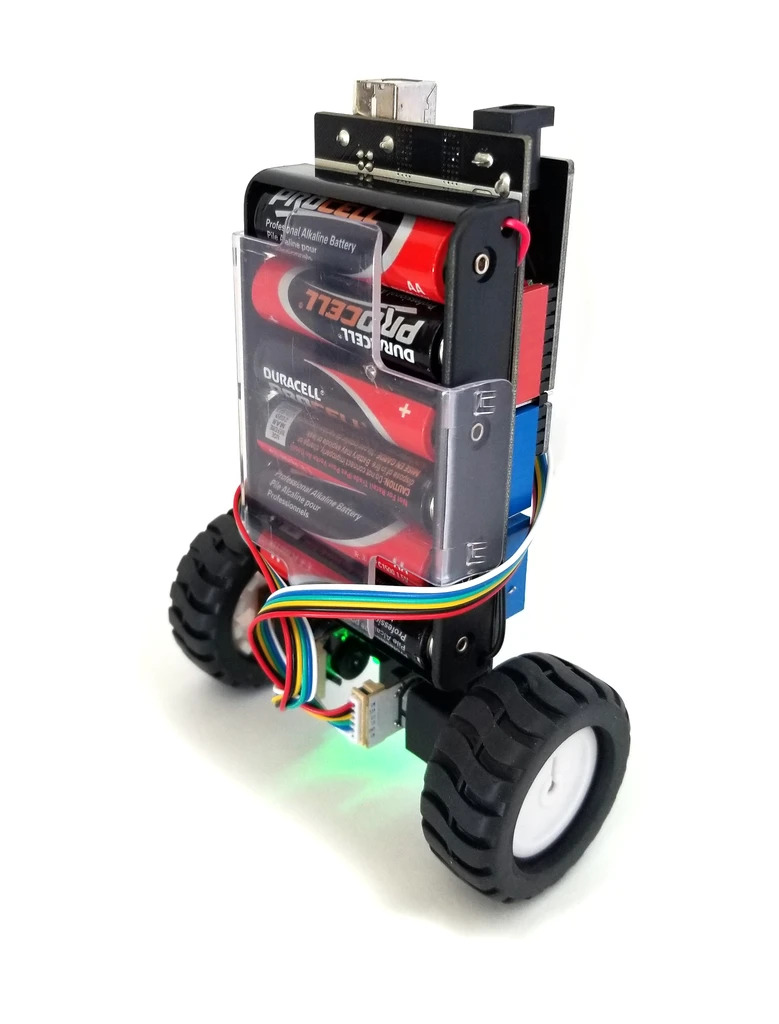
\includegraphics[height = 5.5cm]{minseg-M2V5}
	\end{center}
	\note<1-1>{\begin{itemize}
		\item maybe make Florian do some simple 'voice-music'
	\end{itemize}}
\end{frame}


\setbeamercolor{background canvas}{bg=white!80!black}
\begin{frame}{What are we doing today?}
	\begin{itemize}
		\item show how making the pen stand is similar to making the robot stand
		\item make a demo of a nice pre-made controller that we know it works -- but we won't say how it works at the beginning
		\item we will discover how it works little by little, and eventually discover the simplest, but probably the most important strategy: the P controller!
	\end{itemize}
\end{frame}
\setbeamercolor{background canvas}{bg=white}


\begin{frame}{Our purposes}
	\pause
	\begin{itemize}
		\item have fun
		\pause
		\item understand the world a bit better
		\pause
		\item see that math is useful
	\end{itemize}
\end{frame}


\begin{frame}{What is going to happen in today's part}
	\pause
	\begin{itemize}
		\item connect the pen-balancing and the robot-balancing problems
		\pause
		\item discover together what is the ``P controller''
	\end{itemize}
\end{frame}


\setbeamercolor{background canvas}{bg=white!80!black}
\begin{frame}{Connecting things}
	\begin{itemize}
		\item the robot: this is something that connects to the pen-balancing problem before
		\item also the robot tips
		\item but then the wheels act like the hands!
		\item so the intuition is to make the wheels spin as one would move the hands
		\item but just a moment: when we were balancing the pen we were first of all seeing what was happening, and then also thinking at what to do!
		\item where are the eyes here? and where is the brain?
	\end{itemize}
\end{frame}
\setbeamercolor{background canvas}{bg=white}


\begin{frame}{Connecting the robot with the pen - a small recap, first}{The case of the shower}
	\begin{center}
		\begin{tikzpicture}
			[
				myblock/.style = {draw, rectangle, thick, rounded corners, minimum height = 1.8cm, minimum width = 3.2cm},
				myvariable/.style = {},
				myarrow/.style = {rounded corners, -latex, thick}
			]
			%
			\node (plant) [myblock] {you under the shower};
			%
			\node (output) [myvariable, right = 3cm of plant.east] {how you feel};
			\draw [myarrow] (plant) -- (output) node (auxnode) [coordinate, pos = 0.5] {};
			%
			\node (controller) [myvariable, below = 2cm of plant] {your brain};
			\draw [myarrow] (auxnode) |- (controller);
			%
			\node (actuator) [myvariable, left = 2cm of plant.west] {the knob};
			\draw [myarrow] (controller) -| (actuator);
			%
			\draw [myarrow] (actuator) -- (plant);
			%
		\end{tikzpicture}
	\end{center}
\end{frame}


\begin{frame}{Connecting the robot with the pen - a small recap, first}{The case of the balancing pen}
	\begin{center}
		\begin{tikzpicture}
			[
				myblock/.style = {draw, rectangle, thick, rounded corners, minimum height = 1.8cm, minimum width = 3.2cm},
				myvariable/.style = {},
				myarrow/.style = {rounded corners, -latex, thick}
			]
			%
			\node (plant) [myblock] {the pen on your hand};
			%
			\node (output) [myvariable, right = 3cm of plant.east] {what you see};
			\draw [myarrow] (plant) -- (output) node (auxnode) [coordinate, pos = 0.5] {};
			%
			\node (controller) [myvariable, below = 2cm of plant] {your brain};
			\draw [myarrow] (auxnode) |- (controller);
			%
			\node (actuator) [myvariable, left = 2cm of plant.west] {your hand};
			\draw [myarrow] (controller) -| (actuator);
			%
			\draw [myarrow] (actuator) -- (plant);
			%
		\end{tikzpicture}
	\end{center}
\end{frame}


\begin{frame}{Connecting the robot with the pen - what is what}
	\centering
	\begin{tabular}{p{0.4\textwidth}|p{0.4\textwidth}}
		\ItPrimary{you} & \ItPrimary{the robot} \\
		\pause
		your hands & the wheels (and the motors) \\
		\pause
		your eyes & sensors that measure ``how tilted'' \\
		\pause
		your brain & a small embedded computer \\
	\end{tabular}
\end{frame}


\setbeamercolor{background canvas}{bg=white!80!black}
\begin{frame}{What is what}
	\begin{itemize}
		\item let's see what is what in the robot
		\item the wheels are these ones
		\item the motors are these ones
		\item the sensors are these ones - there are similar ones in the smartphones
		\item the embedded computer is this one
		\item all the rest is stuff that is needed to bring the power here and there
		\item if you find this fascinating then consider becoming a electronics engineer!
	\end{itemize}
\end{frame}
\setbeamercolor{background canvas}{bg=white}


\begin{frame}{The robot as a block scheme}
	\begin{center}
		\begin{tikzpicture}
			[
				myblock/.style = {draw, rectangle, thick, rounded corners, minimum height = 1.8cm, minimum width = 3.2cm},
				myvariable/.style = {},
				myarrow/.style = {rounded corners, -latex, thick}
			]
			%
			\node (plant) [myblock] {the robot};
			%
			\node (output) [myvariable, right = 3cm of plant.east] {the angle};
			\draw [myarrow] (plant) -- (output) node (auxnode) [coordinate, pos = 0.5] {};
			%
			\node (controller) [myvariable, below = 2cm of plant] {the robot's computer};
			\draw [myarrow] (auxnode) |- (controller);
			%
			\node (actuator) [myvariable, left = 2cm of plant.west] {the motors and wheels};
			\draw [myarrow] (controller) -| (actuator);
			%
			\draw [myarrow] (actuator) -- (plant);
			%
		\end{tikzpicture}
	\end{center}
	\note<1-1>{\begin{itemize}
		\item say that what we need to do is to create a 'brain' to be put inside the computer, a brain that understands how to move the motors and wheels given what the robot measures
	\end{itemize}}
\end{frame}


\setbeamercolor{background canvas}{bg=white!80!black}
\begin{frame}{What is what}
	\begin{itemize}
		\item but now I have been talking too much!
		\item let's do as following: now I give you a pre-made brain, and we see if this brain work
		\item I don't tell you how I have created it, I just want you to try it so to see if things work and get something moving
	\end{itemize}
\end{frame}
\setbeamercolor{background canvas}{bg=white}


\begin{frame}{Tryout pause!}
	\begin{itemize}
		\item follow the instructions in the ``tryout A'' manual
		\item does the robot stand on its own?
	\end{itemize}
\end{frame}


\setbeamercolor{background canvas}{bg=white!80!black}
\begin{frame}{post-experience discussion}
	\begin{itemize}
		\item hope things worked!
		\item so now let's discover the most important part of the brain we just inserted in the computer, the famous ``P controller''
		\item we will arrive at it little by little, listing and testing some heuristics control strategies, and eventually arriving to the P controller
	\end{itemize}
\end{frame}
\setbeamercolor{background canvas}{bg=white}


\begin{frame}{A first heuristic}
	\pause
	\begin{center}
		\begin{tikzpicture}
			[
				body/.style = {rectangle, minimum width = 0.7cm, minimum height = 2.4cm, rounded corners, fill = black},
				wheel/.style = {circle, minimum size = 1.4cm, thick, fill = black!50!white, draw = black},
			]
			\node (body) [body] {};
			\node (wheel) [wheel] at (body.south) {};
		\end{tikzpicture} \\
		$\implies$ do nothing
	\end{center}
\end{frame}


\begin{frame}{A first heuristic}
	\begin{center}
		\begin{tikzpicture}
			[
				body/.style = {rectangle, minimum width = 0.7cm, minimum height = 2.4cm, rounded corners, fill = black},
				wheel/.style = {circle, minimum size = 1.4cm, thick, fill = black!50!white, draw = black},
			]
			\node (body) [body, rotate = -30] {};
			\node (wheel) [wheel] at (body.south) {};
		\end{tikzpicture} \\
		$\implies$ spin the wheels as fast as possible clockwise
	\end{center}
\end{frame}


\begin{frame}{A first heuristic}
	\begin{center}
		\begin{tikzpicture}
			[
				body/.style = {rectangle, minimum width = 0.7cm, minimum height = 2.4cm, rounded corners, fill = black},
				wheel/.style = {circle, minimum size = 1.4cm, thick, fill = black!50!white, draw = black},
			]
			\node (body) [body, rotate = 30] {};
			\node (wheel) [wheel] at (body.south) {};
		\end{tikzpicture} \\
		$\implies$ spin the wheels as fast as possible counterclockwise
	\end{center}
\end{frame}


\setbeamercolor{background canvas}{bg=white!80!black}
\begin{frame}
	\begin{itemize}
		\item this approach is problematic
		\item this controller is ``too nervous'': as soon as we are not perfectly aligned then it reacts as much as it can
		\item let me show what this means in practice with the problem of making the pen stand
		\item (example)
		\item see? this 'brain', this controller, does not have too much sense
		\item let's make another heuristic
	\end{itemize}
\end{frame}
\setbeamercolor{background canvas}{bg=white}


\begin{frame}{A second heuristic}
	\begin{center}
		\begin{tikzpicture}
			[
				body/.style = {rectangle, minimum width = 0.7cm, minimum height = 2.4cm, rounded corners, fill = black},
				wheel/.style = {circle, minimum size = 1.4cm, thick, fill = black!50!white, draw = black},
				myline/.style = {dashed, \StrongPrimary, thick},
			]
			\node (body) [body, rotate = -5] {};
			\node (wheel) [wheel] at (body.south) {};
			\draw [myline] (wheel) -- ++(0,3);
			\draw [myline] (wheel) -- ++(0.3,2.7);
			\draw [myline] (wheel) -- ++(0.6,2.3);
		\end{tikzpicture} \\
		$\implies$ depending on the zone, spin the wheels more or less fast
	\end{center}
\end{frame}


\setbeamercolor{background canvas}{bg=white!80!black}
\begin{frame}
	\begin{itemize}
		\item also this approach is a bit problematic
		\item when the system is traversing the transition zones the behavior is 'bumpy': sudden increase, sudden decrease
		\item did you ever went in a car with somebody that drives turning the wheel like in this way? It is kind of a similar thing, you see what I mean? And it is not so comfortable, true?
		\item I would say i prefer somebody that drives smoothly, that moves the wheel in a fluid way, without abrupt changes 
		\item and this is the intuition that leads us to the P controller
	\end{itemize}
\end{frame}
\setbeamercolor{background canvas}{bg=white}


\begin{frame}{The P (i.e., proportional) controller}
	\begin{center}
		\begin{tikzpicture}
			[
				body/.style = {rectangle, minimum width = 0.7cm, minimum height = 2.4cm, rounded corners, fill = black},
				wheel/.style = {circle, minimum size = 1.4cm, thick, fill = black!50!white, draw = black},
				myline/.style = {dashed, \StrongPrimary, thick},
			]
			\node (body) [body, rotate = -5] {};
			\node (wheel) [wheel] at (body.south) {};
			\draw [myline] (wheel) -- ++(0,3);
		\end{tikzpicture} \\
		$\implies$ speed of the wheels = $P \cdot $ angular error
	\end{center}
	\note<1-1>{\begin{itemize}
		\item make clear that $P$ is a design choice
	\end{itemize}}
\end{frame}


\setbeamercolor{background canvas}{bg=white!80!black}
\begin{frame}
	\begin{itemize}
		\item but how do we design $P$?
		\item to understand we should ask ourselves: what is the effect of having different $P$s?
		\item if I put $P = $ a tiny tiny number, what is going to happen?
		\item if I put $P = $ a huge number, what is going to happen?
		\item let's have a chat all together, and see what we think about this
	\end{itemize}
\end{frame}
\setbeamercolor{background canvas}{bg=white}


\begin{frame}{Discussion pause!}
	\begin{itemize}
		\item if I put $P = $ a tiny tiny number, what is going to happen?
		\item if I put $P = $ a huge number, what is going to happen?
	\end{itemize}
\end{frame}


\setbeamercolor{background canvas}{bg=white!80!black}
\begin{frame}
	\begin{itemize}
		\item amazing, I am proud of your chatting!
		\item but I will leave you with a cliffhanger; we are going to discuss the effects of choosing $P$ in the next part
		\item so, be ready to move to the next part of the experience! See you in 'part 3', where we add two ingredients to this controller, and then make our own version of the robot brain!
	\end{itemize}
\end{frame}
\setbeamercolor{background canvas}{bg=white}


% ~~~~~~~~~~~~~~~~~~~~~~~~~~~~~~~~~~~~~~~~~~~~~~~~~~~~~~~~~~~~~~~~~ %
\end{document}														%
% ~~~~~~~~~~~~~~~~~~~~~~~~~~~~~~~~~~~~~~~~~~~~~~~~~~~~~~~~~~~~~~~~~ %
% ./FramesTemplates/template__citation.tex
% ./FramesTemplates/template__empty_frame.tex
% ./FramesTemplates/template__frame_with_blocks.tex
% ./FramesTemplates/template__frame_with_colored_background.tex
% ./FramesTemplates/template__frame_with_itemized_list.tex
% ./FramesTemplates/template__frame_with_overlayed_figures.tex
% ./FramesTemplates/template__frame_with_two_columns.tex
% ./FramesTemplates/template__frame_with_two_columns_and_overlayed_figures.tex


\begin{frame}{<++>}{<++>}
	<++>
	\note<1-1>{\begin{itemize}
		\item <++>
	\end{itemize}}
\end{frame}
<++>


